% Component Error Variance Decomposition (Player Props)
% Replaces: tab:variance-decomposition in section_dirichlet_stacking.tex
% Stacked horizontal bar showing within-player vs opponent variance

\begin{figure}[htbp]
\centering
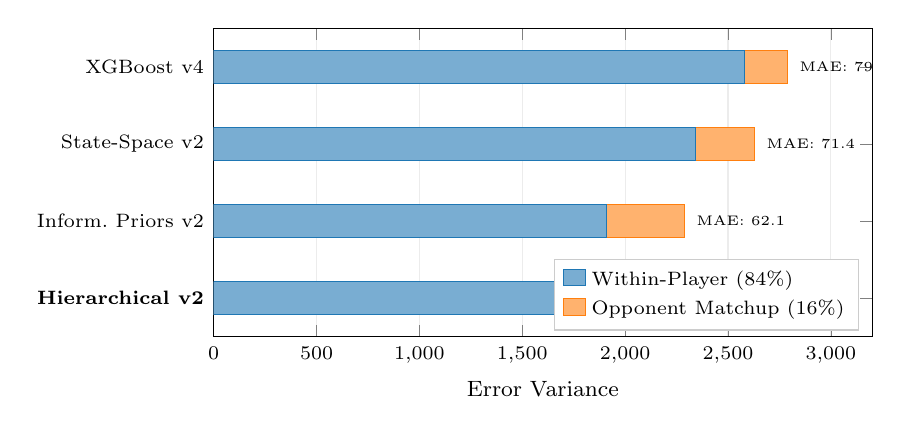
\begin{tikzpicture}
\definecolor{colWithin}{RGB}{31,119,180}
\definecolor{colOpp}{RGB}{255,127,14}

\begin{axis}[
  width=0.82\textwidth,
  height=5.5cm,
  xbar stacked,
  bar width=12pt,
  xlabel={Error Variance},
  xlabel style={font=\footnotesize},
  xmin=0, xmax=3200,
  ytick={1,2,3,4},
  yticklabels={
    XGBoost v4,
    State-Space v2,
    {Inform.\ Priors v2},
    {\textbf{Hierarchical v2}}
  },
  yticklabel style={font=\scriptsize},
  y dir=reverse,
  xticklabel style={font=\scriptsize},
  legend style={at={(0.98,0.02)}, anchor=south east, font=\scriptsize, draw=gray!40, cells={anchor=west}},
  grid=major,
  grid style={gray!15},
  ymajorgrids=false,
  enlarge y limits={abs=0.5},
]

% Within-player variance
\addplot[fill=colWithin!60, draw=colWithin] coordinates {
  (2580, 1) (2340, 2) (1910, 3) (1820, 4)
};
\addlegendentry{Within-Player (84\%)}

% Opponent variance
\addplot[fill=colOpp!60, draw=colOpp] coordinates {
  (210, 1) (290, 2) (380, 3) (340, 4)
};
\addlegendentry{Opponent Matchup (16\%)}

% MAE labels
\node[font=\tiny, anchor=west] at (axis cs:2800,1) {MAE: 79.8};
\node[font=\tiny, anchor=west] at (axis cs:2640,2) {MAE: 71.4};
\node[font=\tiny, anchor=west] at (axis cs:2300,3) {MAE: 62.1};
\node[font=\tiny\bfseries, anchor=west] at (axis cs:2170,4) {MAE: 58.3};

\end{axis}
\end{tikzpicture}
\caption[Variance decomposition by component]{Error variance decomposition for player passing predictions. Within-player variance (blue, 84\% of total) dominates opponent matchup effects (orange, 16\%). Hierarchical v2 minimizes within-player variance (1820 vs.\ XGBoost's 2580), explaining its dominant 39.6\% Dirichlet weight. XGBoost minimizes opponent variance (210) but this signal is comparatively small for props.}
\label{fig:variance-decomposition-chart}
\end{figure}
